\documentclass{article}
\usepackage{graphicx} % Required for inserting images
\usepackage{todonotes}
\usepackage[colorlinks=true, allcolors=blue]{hyperref}
\usepackage{biblatex}
\addbibresource{references.bib}

\newcommand\todoJason[1]{\todo[author=Jason,color=yellow,inline]{#1}}
\newcommand\todoMichael[1]{\todo[author=Michael,color=green,inline]{#1}}
\newcommand\todoChris[1]{\todo[author=Chris,color=orange,inline]{#1}}

\title{Progress Report: How Super are Super Computers?}
\author{Jason Stewart\\
\textit{jastewart@unm.edu} 
\and
Michael Servilla\\
\textit{chico@unm.edu}
\and
Christopher Leap\\
\textit{cleap@unm.edu}
\date{\today}
}

\begin{document}

\maketitle
\section{Current progress}
At the time of this report, we have written and run our all\_to\_all and count\_primes benchmarks on seven different machines. These machines are a combination of our personal computers and the CS machines at the University of New Mexico (UNM). We ran each benchmark using 1, 2, 4, 6, 8, 16, 32, 64, and 128 processes. For each run, we calculated the average and standard deviation of the amount of time to took to run one iteration of MPI\_Alltoall with a message size of 4196 bytes or one iteration of each process counting prime numbers between 0 and 10000 and performing a single MPI\_Allgather at the end. The GitHub repository for our project is included in our References section \cite{repo}. Preliminary results are included at the end of this report.

\section{Challenges}
We encountered unexpected difficulty running oversubscribed jobs on the CARC supercomputers. We have found a workaround to let us oversubscribe CARC nodes but creating this method delayed our results from CARC systems.

\section{Future Work}
The following work remains to be completed:
\begin{enumerate}
    \item Run our benchmarks on CARC systems.
    \item Analyze our results across the following metrics:
    \begin{enumerate}
        \item Plot average runtime versus number of processes.
        \item Compute and plot normalized time versus  number of processes. Normalized time will be calculated by multiplying average runtime by the clock speed of the processor.
        \item Compute and plot average runtime versus normalized cores. Normalized cores will be calculated by multiplying average runtime by number of cores available divided by the number of processes used.
        \item Plot normalized time by normalized cores.
    \end{enumerate}
    \begin{enumerate}
        \item These plots will indicate if network bandwidth is a limiting factor in our benchmarks or if there are other variables that effect runtime besides clock speed and number of cores on a processor.
    \end{enumerate}
    \item Formalize these findings in a written report.
\end{enumerate}

\printbibliography

\section{Preliminary Results}

We ran the ``all\_to\_all" and ``count\_primes" benchmarks for each of the computers. We ran each benchmark 800 times. For Figures 1 through 4, each line corresponds to the mean across the 800 runs with the shaded area corresponding to one standard deviation either side of the mean. Figure \ref{fig:all_to_all} and Figure \ref{fig:count_primes} show the results of the benchmarks using the timings directly. 

For Figure \ref{fig:all_to_all_normalized} and Figure \ref{fig:count_primes_normalized}, we attempt to ``normalize" the results by multiplying each benchmark timing (seconds per benchmark) by the computer's clock speed (cycles per second) to get the timings in cycles per benchmark. 

In Figure \ref{fig:all_to_all_scaled} and Figure \ref{fig:count_primes_scaled}, we compare each computer's performance using a scaled metric - we multiply each benchmark time by the number of processes used and divide by the total number of cpu cores on the computer. 

\begin{figure}[h]
    \centering
    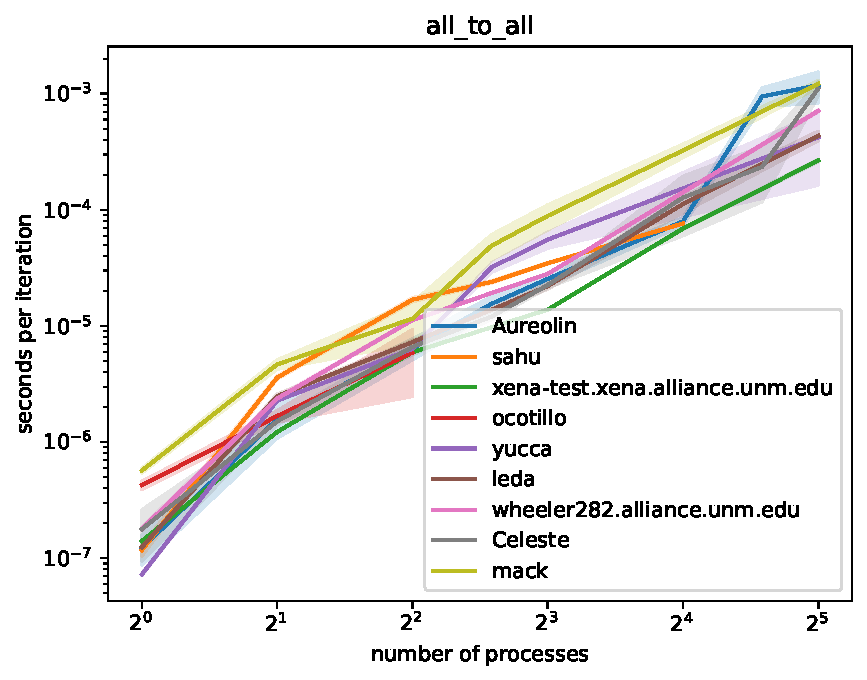
\includegraphics[width=0.8\textwidth]{figures/draft/all_to_all.pdf}
    \caption{}
    \label{fig:all_to_all}
\end{figure}

\begin{figure}[h]
    \centering
    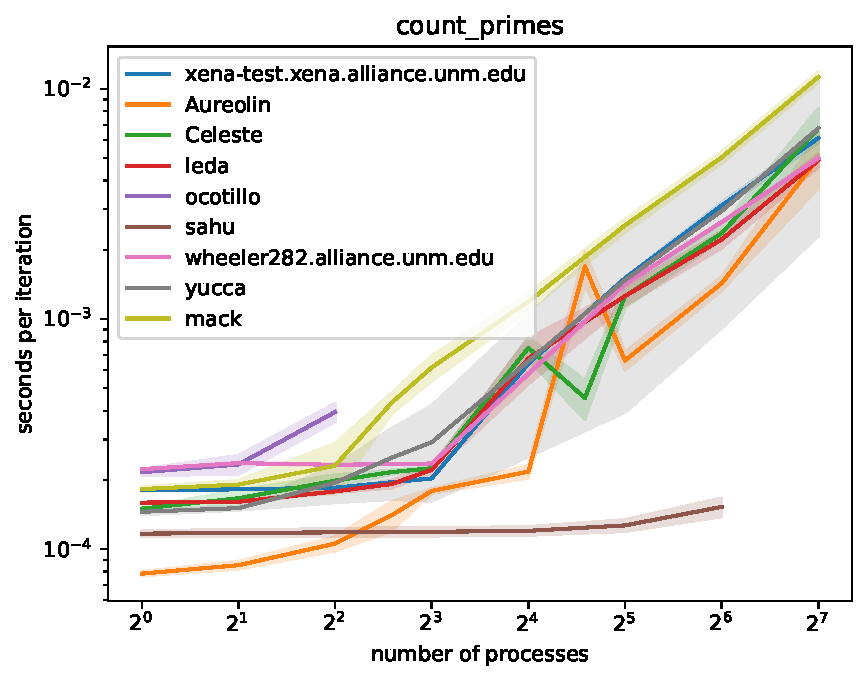
\includegraphics[width=0.8\textwidth]{figures/draft/count_primes.pdf}
    \caption{Caption}
    \label{fig:count_primes}
\end{figure}

\begin{figure}[h]
    \centering
    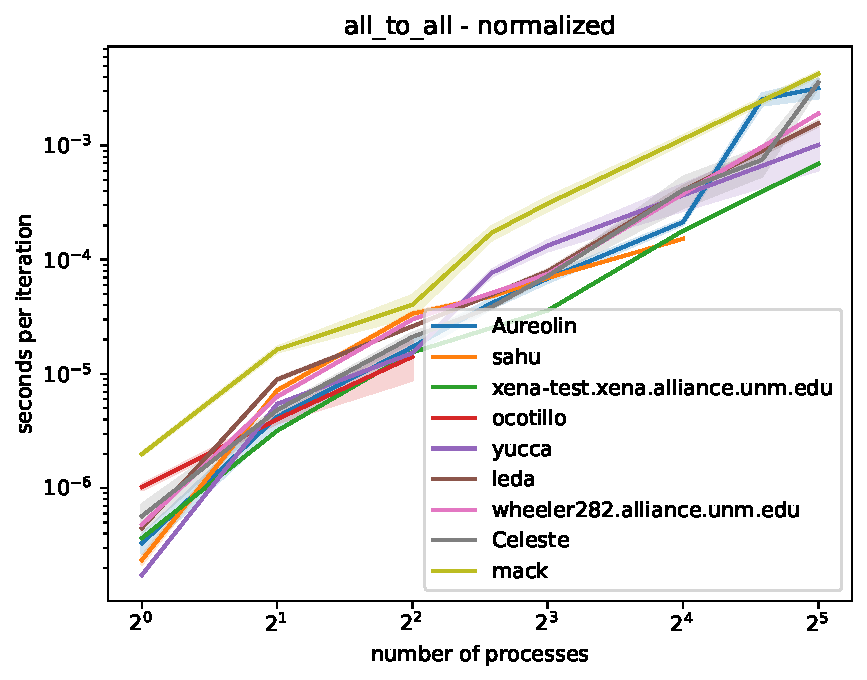
\includegraphics[width=0.8\textwidth]{figures/draft/all_to_all_normalized.pdf}
    \caption{Caption}
    \label{fig:all_to_all_normalized}
\end{figure}

\begin{figure}[h]
    \centering
    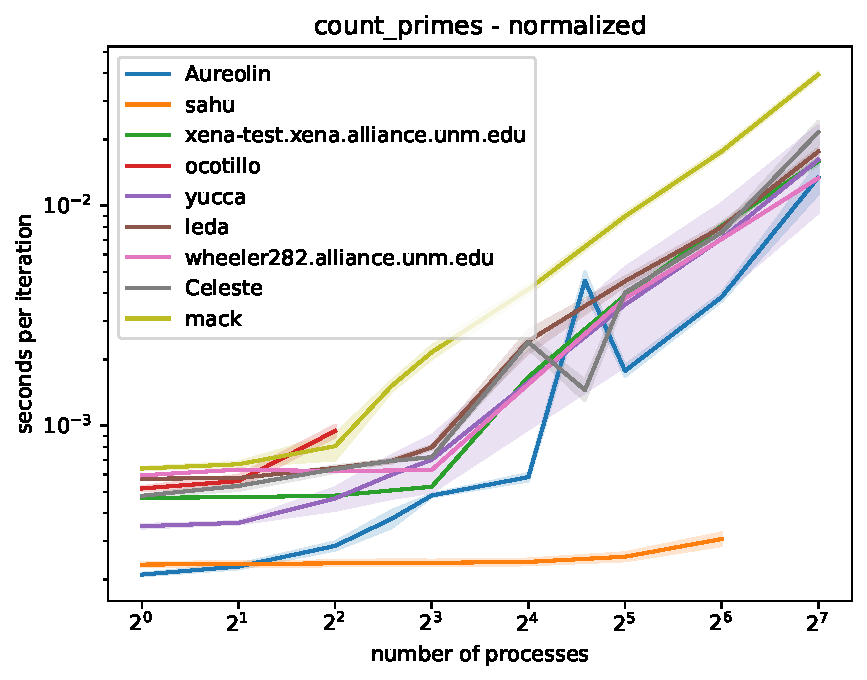
\includegraphics[width=0.8\textwidth]{figures/draft/count_primes_normalized.pdf}
    \caption{Caption}
    \label{fig:count_primes_normalized}
\end{figure}

\begin{figure}[h]
    \centering
    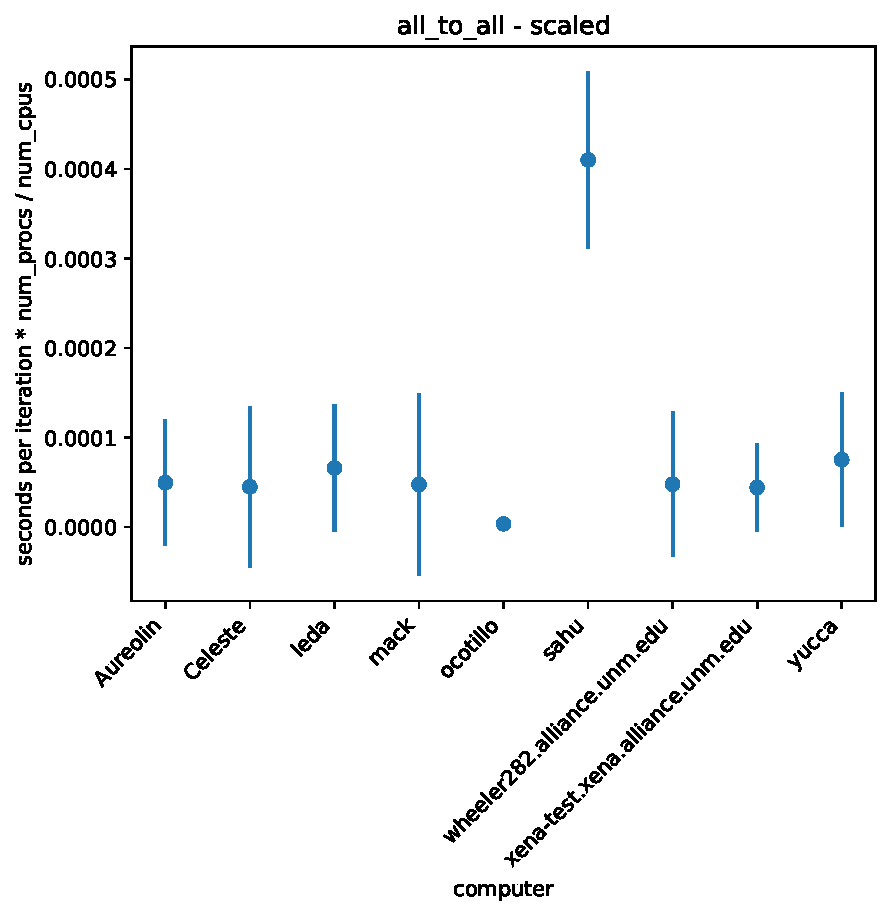
\includegraphics[width=0.8\textwidth]{figures/draft/all_to_all_scaled.pdf}
    \caption{Caption}
    \label{fig:all_to_all_scaled}
\end{figure}

\begin{figure}[h]
    \centering
    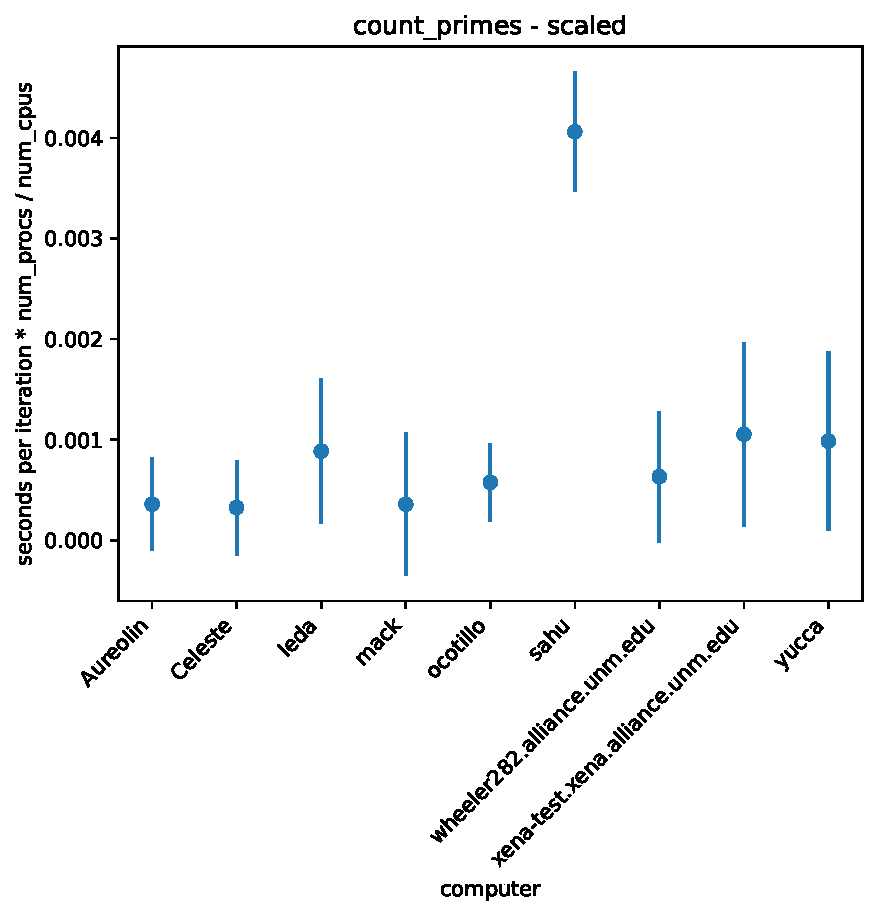
\includegraphics[width=0.8\textwidth]{figures/draft/count_primes_scaled.pdf}
    \caption{Caption}
    \label{fig:count_primes_scaled}
\end{figure}

\begin{figure}[h]
    \centering
    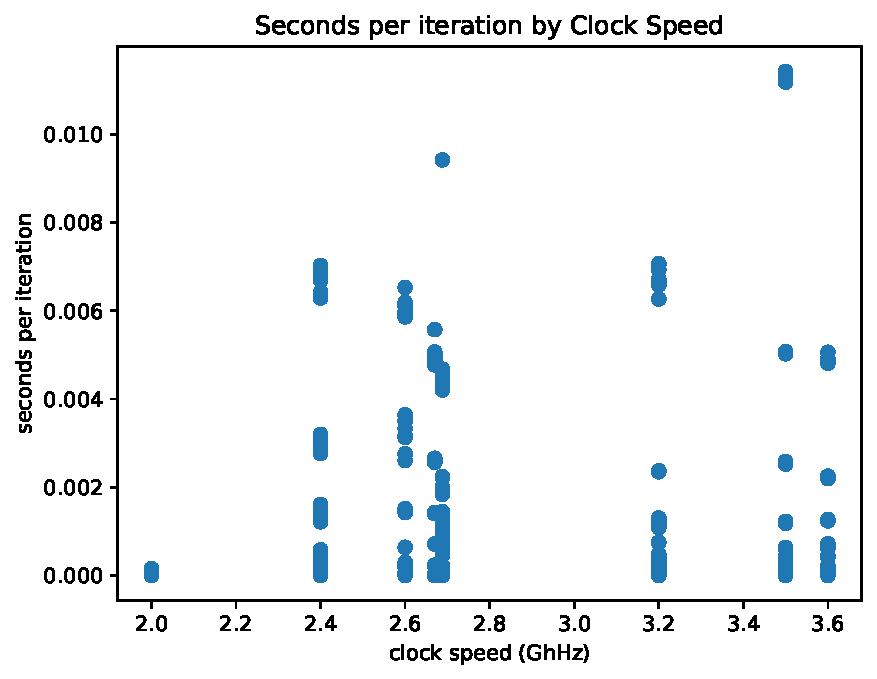
\includegraphics[width=0.8\textwidth]{figures/draft/correlation.pdf}
    \caption{Caption}
    \label{fig:correlation}
\end{figure}


\end{document}

Commands: \\
\textbf{lscpu} \\
if lspcu doesn't give clock speed, try \textbf{cat /proc/cpuinfo | grep Hz} \\

\begin{itemize}
\item Specs format: CPU model (Model name), Cores per node, Cores per socket, clock rate
    \item Hopper: Intel(R) Xeon(R) Gold 6226R, 64, 16, 2.90GHz
    \item Wheeler: Intel(R) Xeon(R) X5550, 8, 4, 2.67GHz
    \item Aureolin (Jason's laptop): 12th Gen Intel(R) Core(TM) i7-12700H, 10, 10, 2688 MHz
    \item Celeste (Jason's desktop): Intel(R) Core(TM) i7-8700, 6, 6, 3200 MHz
    \item Leda (CS machine): Intel(R) Core(TM) i9-9900K, 16, 8, 3.60GHz
    \item Trucks (CS machine): Intel(R) Xeon(R) CPU E5-2637 v4, 4, 1, 3.50GHz
    \item Sahu (TumorAI machine): Intel(R) Xeon(R) Gold 6338, 128, 32, 2.00GHz
    \item Xena: Intel(R) Xeon(R) CPU E5-2640 v3, 16, 8, 2.60GHz
    \item Ocotillo (Servilla's laptop): Intel(R) Core(TM) i7-5500U, 4, 2, 2.40GHz
    \item Yucca (Servilla'a Laptop): Intel(R) Core(TM) i9-10885H, 16, 8, 2.40GHz
\end{itemize}



\printbibliography

\end{document}


example cite: \cite{cfb_db}


\newpage
\nocite{*}
\bibliographystyle{acm}
\bibliography{references}
